\pagebreak
\section{Alloy}
\lstinputlisting[language=alloy]{../alloy/alloy.als}

\pagebreak
\subsection{Output}
Here is the result of Alloy Analyzer for each assert and predicate.

%\vfill
%\includegraphics[scale=0.7]{executionresult.jpg}
%\vfill

\pagebreak
\subsection{Generated Worlds}
Here are presented two generated by Alloy according to the model specification.
The first one shows a rather simple and general case: there are three cars,
one in used by a user and associated to its relative ride,
one reseved by another user and the last one available for reservations.
The first one on the contarary is focused more on the concept of ride history.
We see five rides associated to the same user and to five different cars
but only one if this ride is active, meaning that the car is currently in use and the
others are just kept for backlog. This is stressed by the fact that some of the cars used 
in the previous rides are now reserved again.

\begin{figure}
    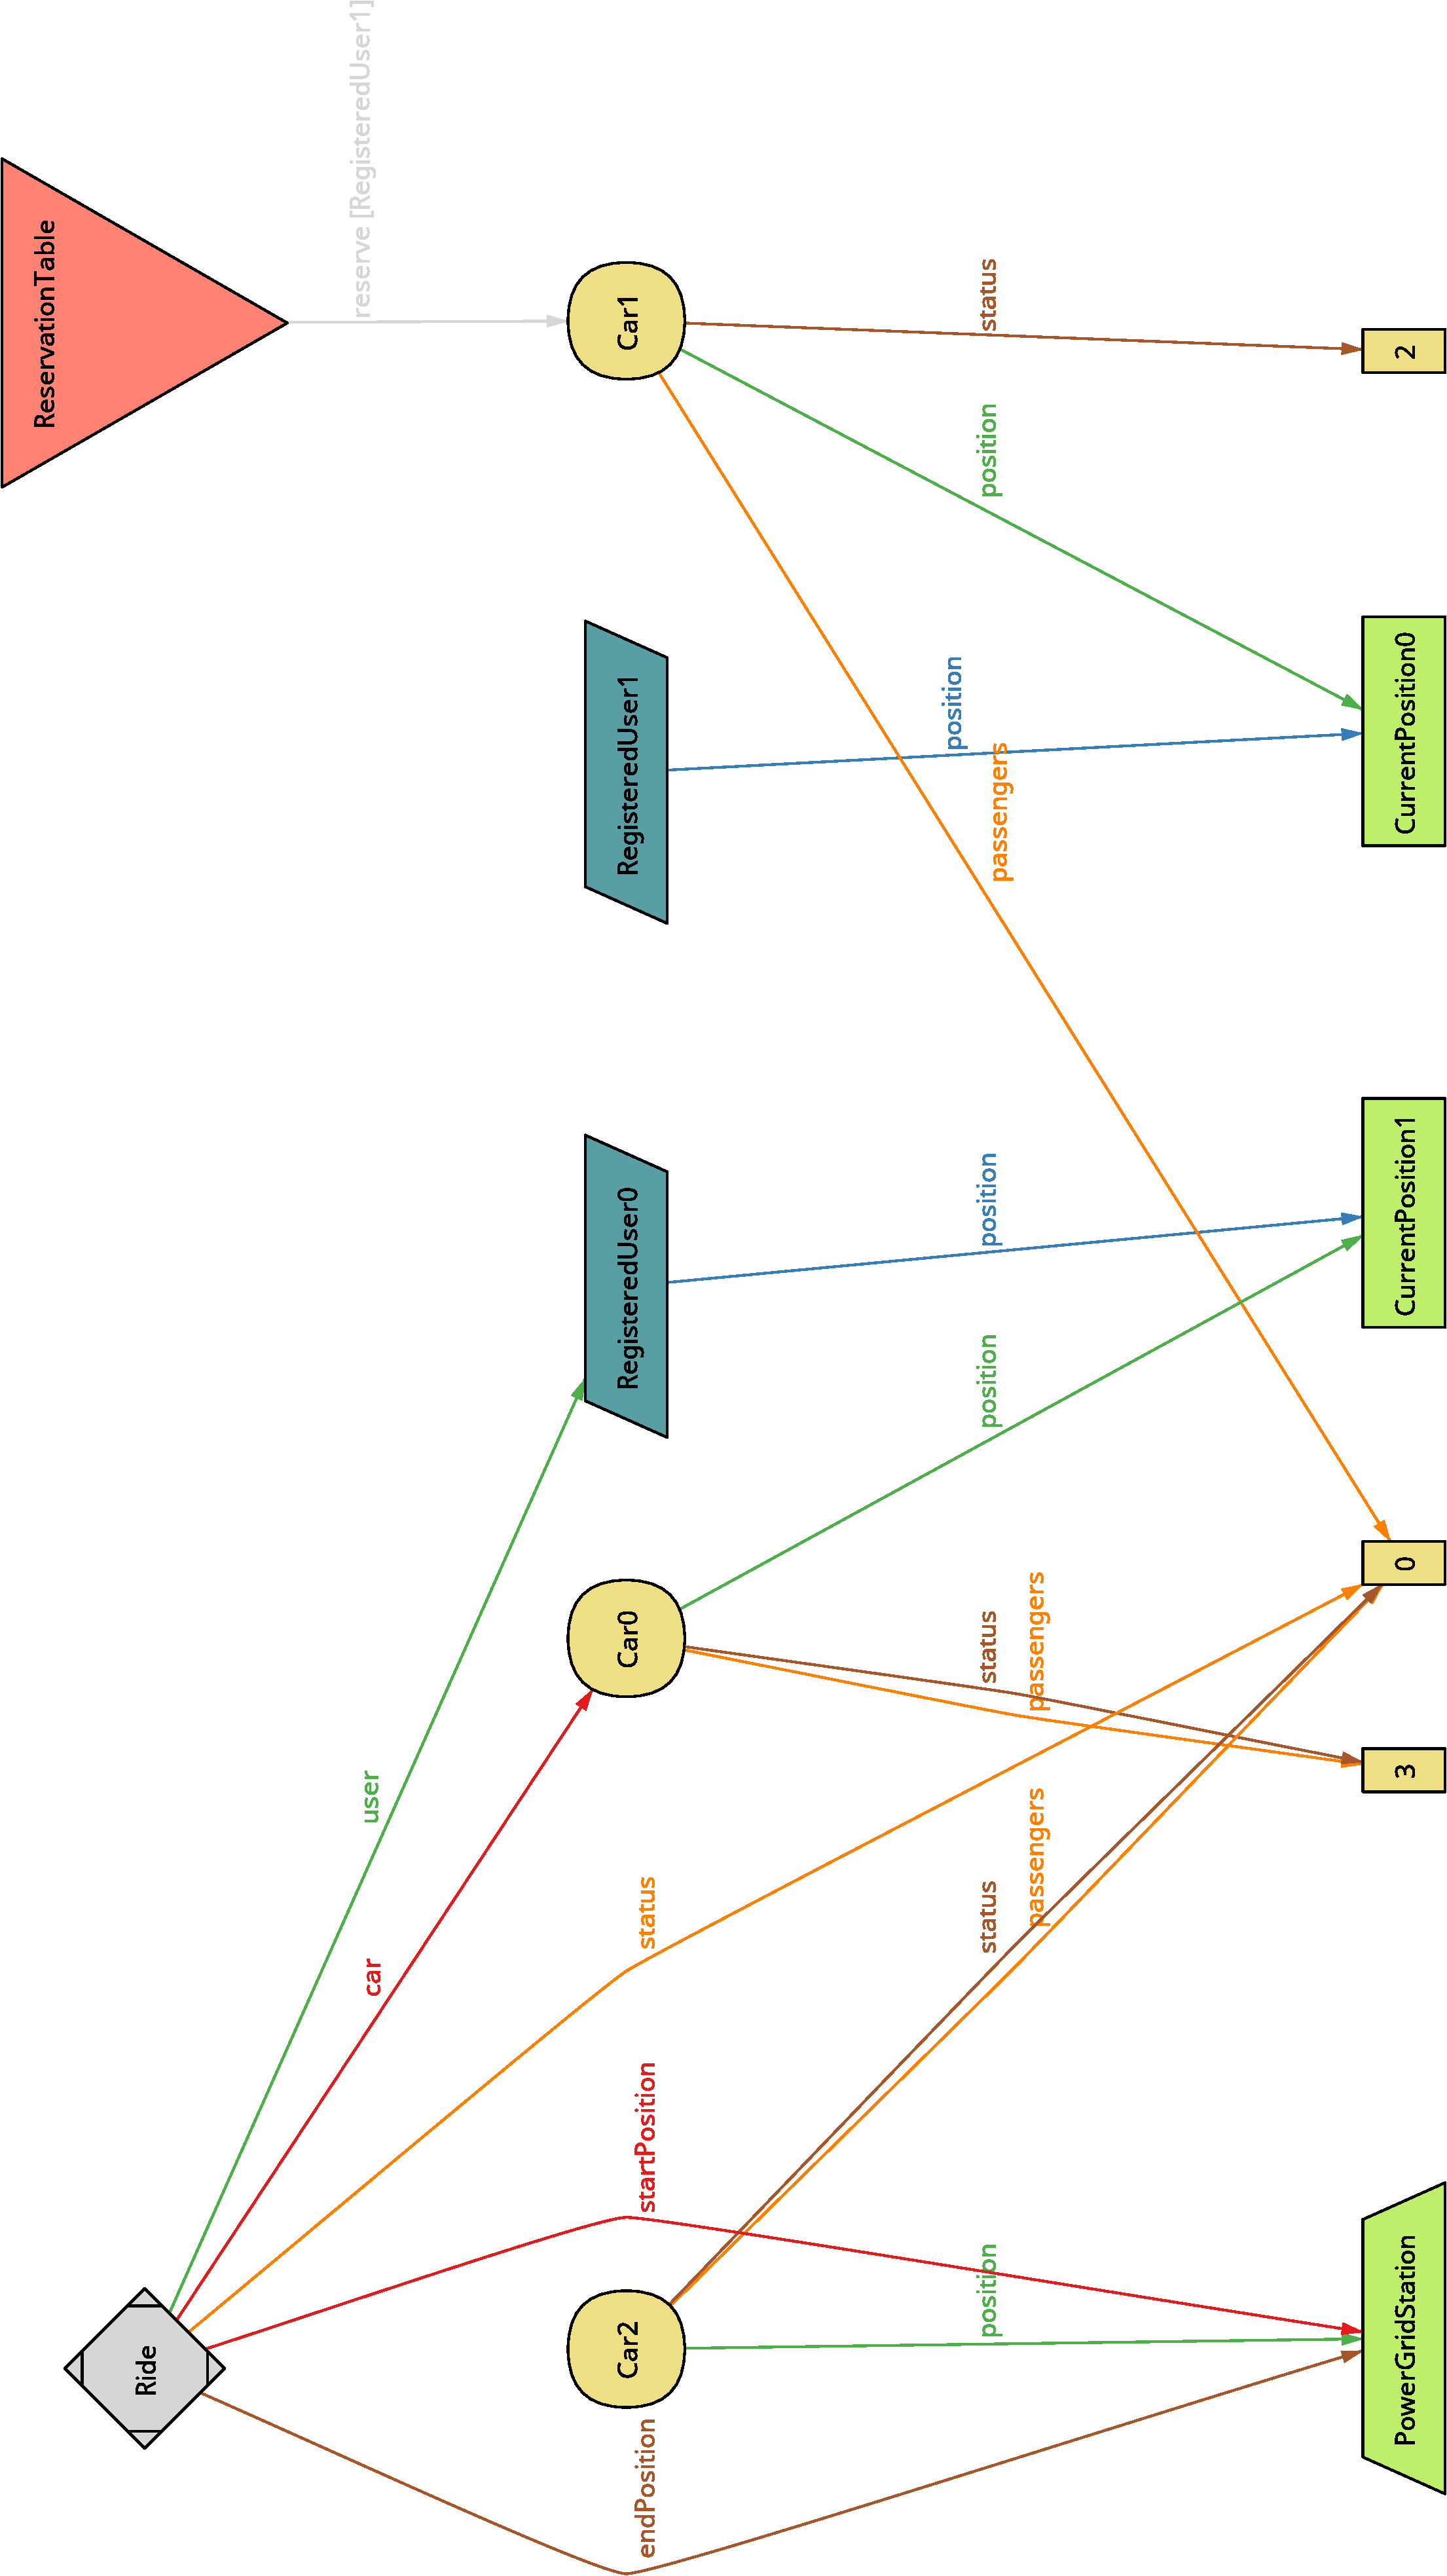
\includegraphics[width=\textwidth,height=0.95\textheight,keepaspectratio]{alloysimple.pdf}
    \caption{Simple Alloy world.}
\end{figure}

\begin{figure}
    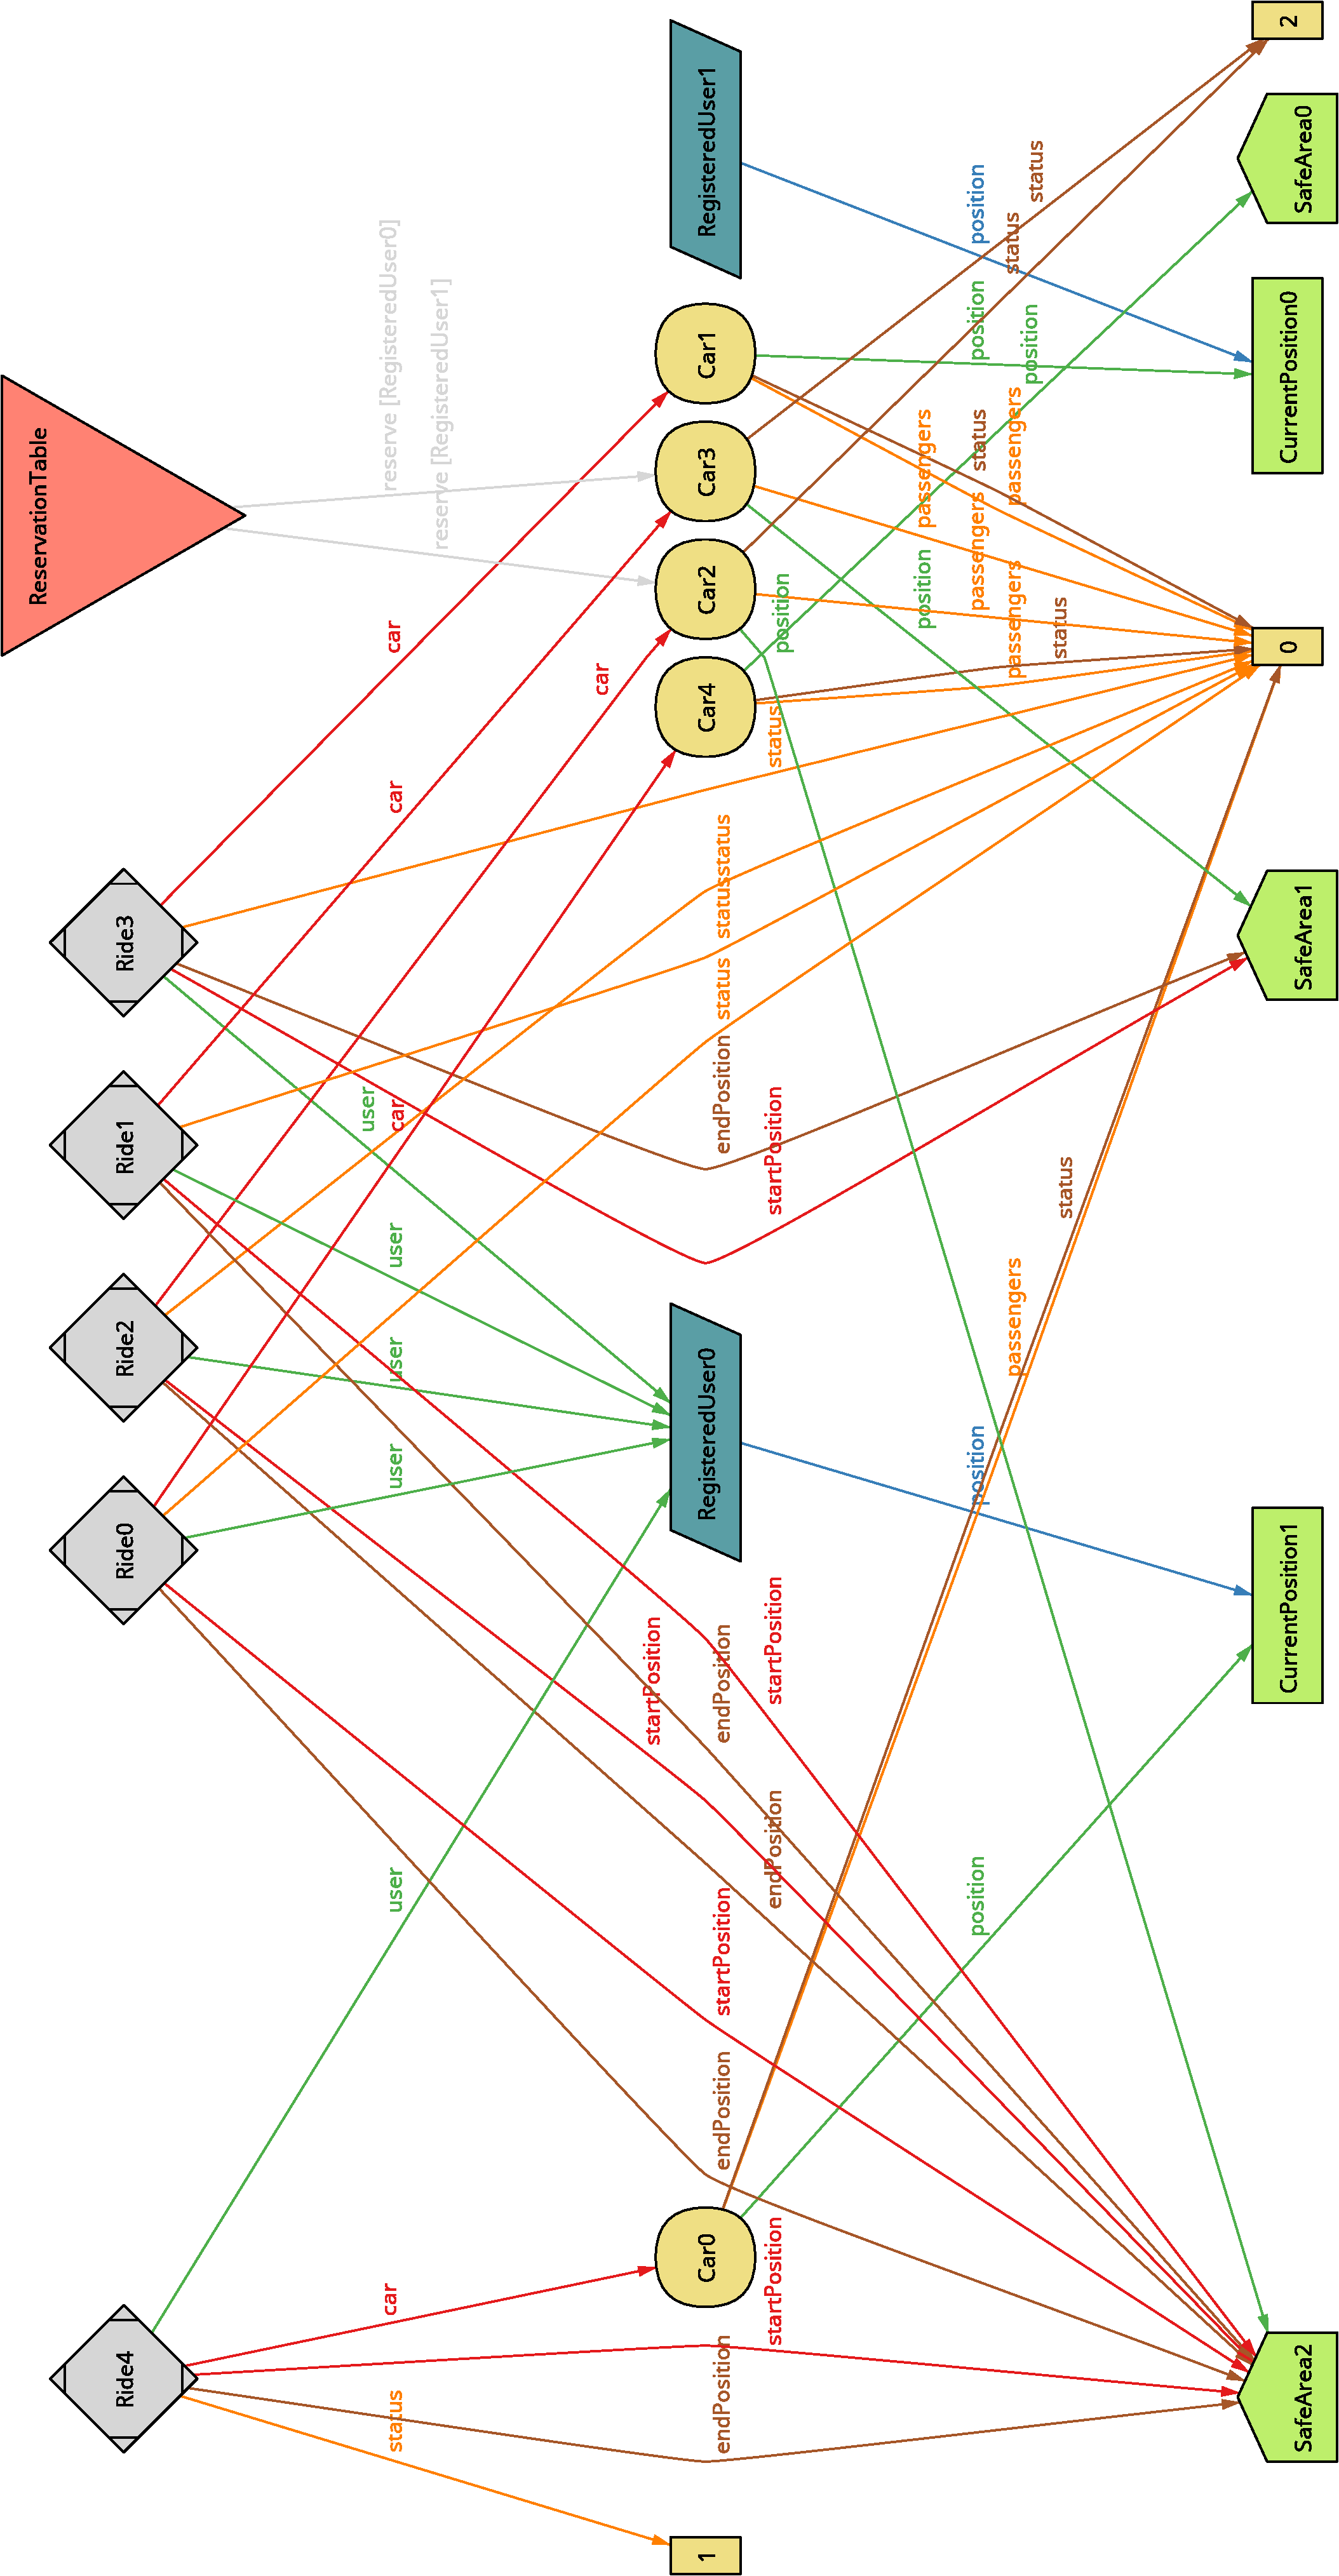
\includegraphics[width=\textwidth,height=0.95\textheight,keepaspectratio]{alloycomplex.pdf}
    \caption{Complex Alloy world with Rides history.}
\end{figure}
